\chapter{The Backend}
\label{backend}
	\section{Introduction}
		\begin{figure}[H]
			\iftrue
			\caption{Backend Services}
			\centering
			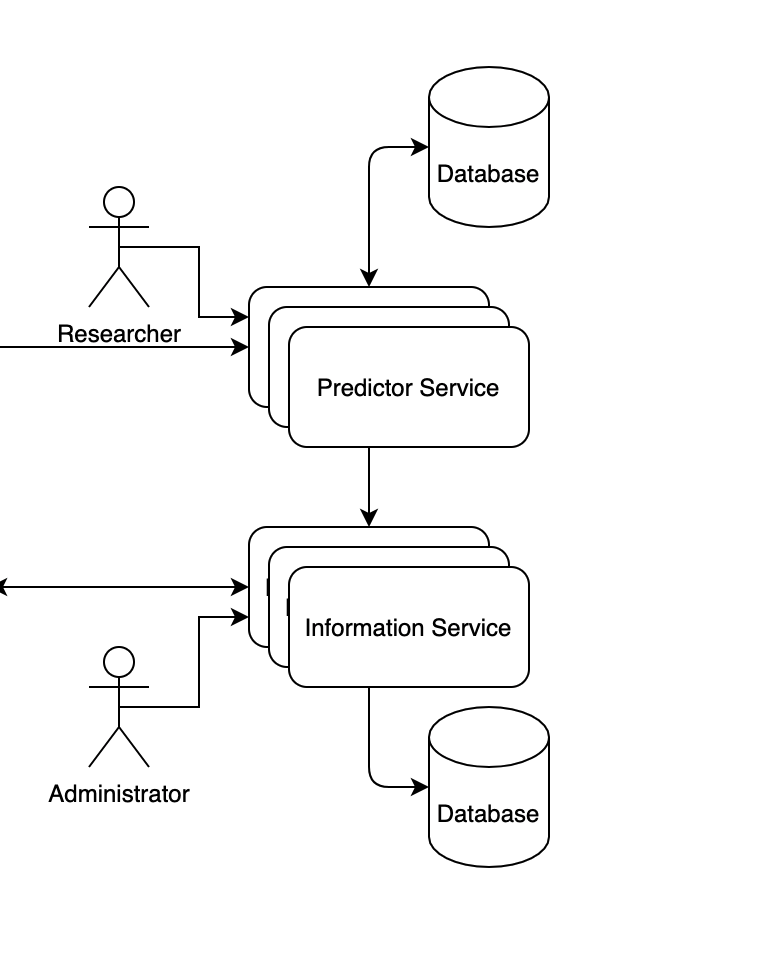
\includegraphics[scale=0.5]{figures/backend}
			\fi
		\end{figure}
		In this chapter we will cover extensively the inner workings of the backend services, namely the Information and the Prediction services
		We will go through their internal architectures as well as some key areas of interest.
	\section{Information Service}
		The Information Service(internally known as uortmc-infobe) is the service that handles the information of our entities, namely the
		patients, the scans, the end-users and their interconnections, additionally it handles authentication and includes the notification
		system, capable of notifying a given end-user for the completion of their tasks.\par
		\subsection{Technology Stack}
			The Information service uses a number of libraries to achieve its goals, the most important ones are listed below
			\begin{itemize}
				\item Django framework
				\item psycopg2 database driver
			\end{itemize}	
			\subsubsection{Django Framework}
				\label{django}
				Django is a free and open-source, python based web framework that uses the model-template-view(MTV) architecture pattern. 
				It is maintained by an american  501(c)(3) non-profit organisation called Django Software Foundation (DSF). Django offers 
				the code infastructure to develop RESTFul[\cite{restful-rfc7231}] microservices with ease, and its the backbone of both of our
				microservices
			\subsubsection{psycopg2 database driver}
				\label{psycopg2}
				psycopg2 is a famous postgres database driver for python. psycopg2 offers the interface for our postgres database connection, 
				implementing the server-client protocol behind the scenes.
		\subsection{Code Architecture}
			The Information service is designed to be a fully Object Oriented Entity[\cite{oop}].
			The architectural design of the Information Service can be seen below.\pagebreak
			\begin{figure}[H]
				\iftrue
				\caption{OOP Diagram}
				\centering
				 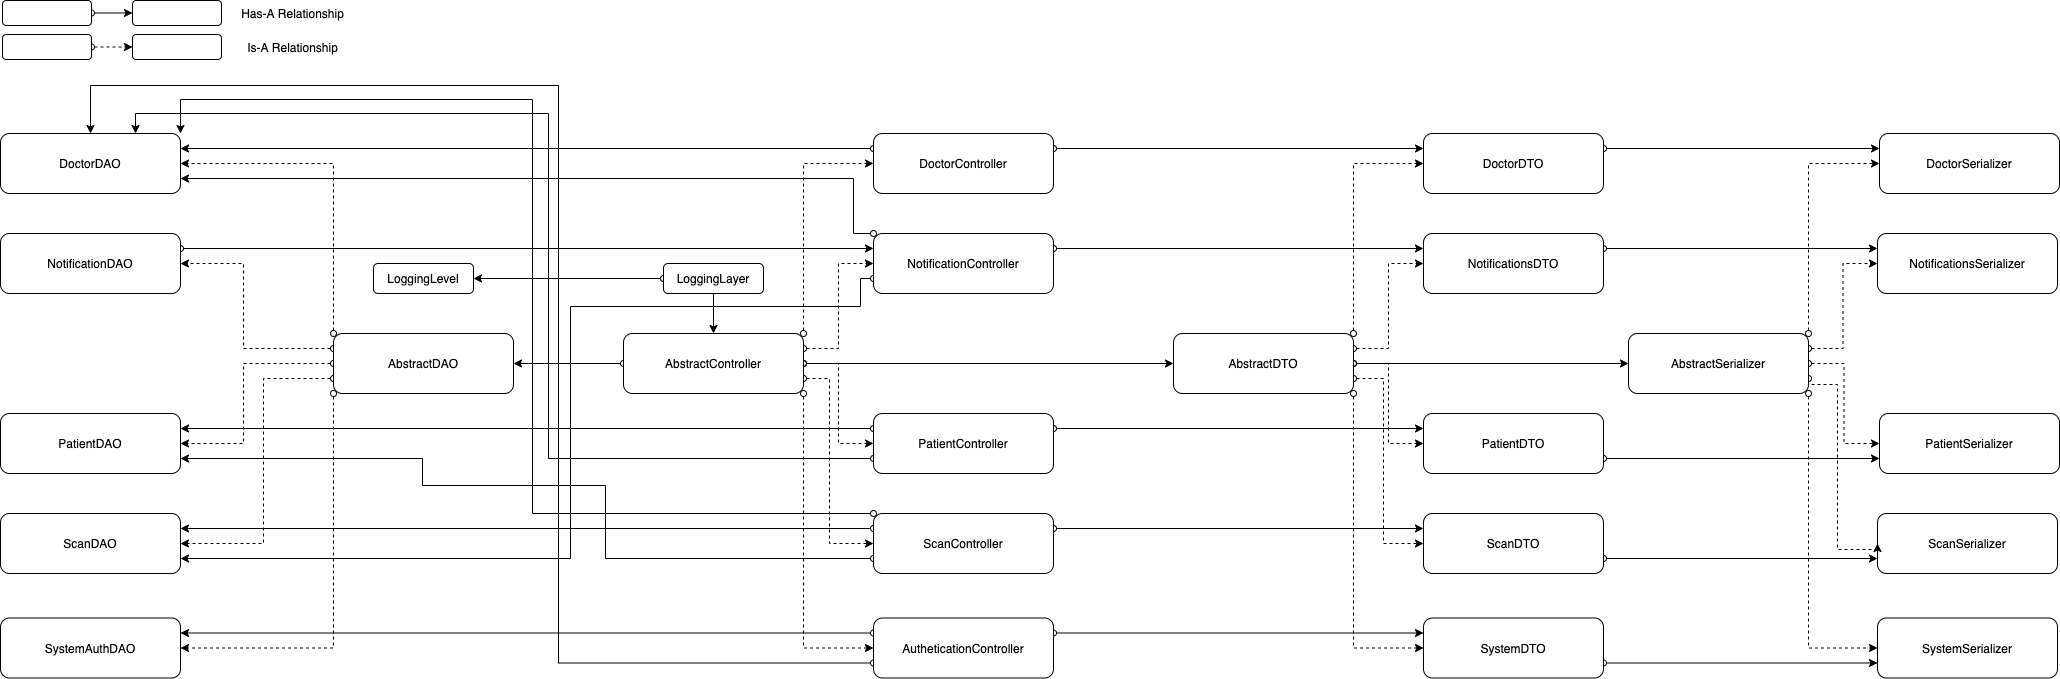
\includegraphics[angle=90,origin=c,scale=0.3]{figures/InformationServiceArchitecture}
				\fi
			\end{figure}\pagebreak
			The entrypoints for the requests, are the following classes
			\begin{itemize}
				\item \textbf{DoctorController}: This Class handles everything related to the Doctor Entity.
				\item \textbf{NotificationController} : This Class handles everything related to the Notification Entity.
				\item \textbf{PatientController} : This Class handles everything related to the Patient Entity.
				\item \textbf{ScanController} : This Class handles everything related to the Scan Entity.
				\item \textbf{AutheticationController} : This Class handles everything related to the Authentication service.
			\end{itemize}
			When a request is sent to the Information service, the proper Class is selected based on the request endpoint and details. 
			Then the respective class will use the rest of the classes services to perform the needed actions and respond to the request
			accordincly. A exhaustive list of the rest major classes are given below.
			\begin{center}
				\begin{tabular}{ |c|c| } 
					\hline
					DoctorDAO & Handles the SQL Queries of Doctor Entity \\
					NotificationDAO & Handles the SQL Queries of Notification Entity  \\\
					PatientDAO & Handles the SQL Queries of the Patient Entity\\
					ScanDAO & Handles the SQL Queries of the Scan Entity\\
					SystemAuthDAO & Handles the SQL Queries of the Authentication service\\
					AbstractDAO & Used to describe any DAO(Data Access Object) available\\
					LoggingLayer & Used by controllers to notify the operator in case of errors\\
					LoggingLevel &Used by LoggingLayer to describe the severity of an error\\
					AbstractController & Used to describe any controller available\\
					AbstractDTO & Used to describe any DTO(Data Transfer Object)'s available\\
					DoctorDTO & The responce objects for Doctor Entities\\
					NotificationsDTO & The responce objects for Notification Entities\\
					PatientDTO & The responce objects for Patient Entities\\
					ScanDTO & The responce objects for Scan Entities\\
					SystemDTO & The responce objects for Authentication Entities\\
					AbstractSerializer & Used to describe any serializer available\\
					DoctorSerializer & Used to convert Doctor DTO responce into JSON\\
					NotificationsSerializer & Used to convert Notification DTO responce into JSON\\
					ScanSerializer & Used to convert Scan DTO responce into JSON\\
					SystemSerializer & Used to convert SystemAuthDTO responce into JSON\\
					\hline
				\end{tabular}
			\end{center}
		\subsection{Database Medium}
			The Information Service uses an RDBMS(Relational Database Managment System)[\cite{friedrichsen_ruffolo_monk_starks_pratt_last_1995}] called Postgres. PostgreSQL is a open-source and 
			free relational database emphasizing on extensibility and SQL standard compliance. The relational diagram of the Information Service
			can be seen below.Additional information relating the E-R Diagram can be found in chapter \ref{entity-relation-analysis} \pagebreak
			\begin{figure}[H]
				\iftrue
				\caption{E-R Diagram}
				\centering
				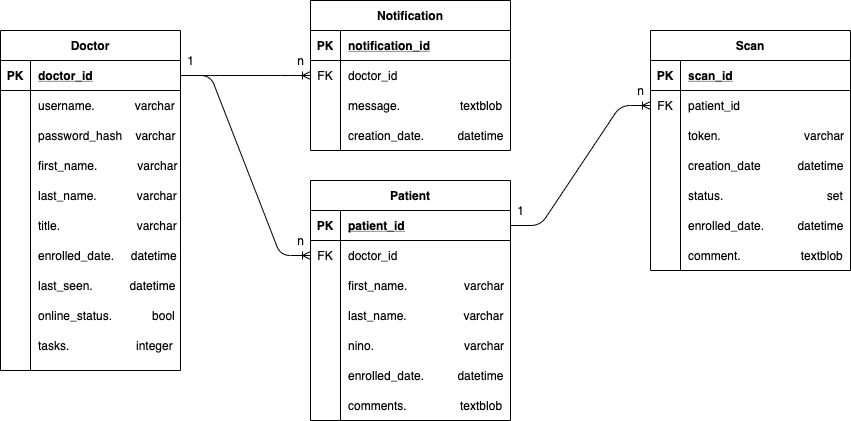
\includegraphics[angle=90,origin=c,scale=0.8]{figures/InformationServiceDatabaseDiagram}
				\fi
			\end{figure}\pagebreak
	
	\section{Prediction Service}
		The Prediction Service(internally known as uortmc-taskbe) is the service that handles the prediction proccess ultrasound images, it has 
		also the responsibility of notifing the end-user when a task is completed, by calling the Information Service's Notification service.
		In this section we will briefly look at the Prediction Service internals, except from the prediction itself. For more information on the
		prediction proccess please refer to chapter \ref{prediction-process}
		\subsection{Technology Stack}
			The Prediction service uses a number of libraries to achieve its goals, the most important ones are listed below
			\begin{itemize}
				\item Django framework (see paragraph \ref{django})
				\item psycopg2 database driver (see paragraph \ref{psycopg2})
				\item base64 decoders
				\item imghdr image library
				\item Pykka actors
			\end{itemize}
			\subsubsection{base64 decoder}
				base64 decoding library is a famous decoding library for python. it offers the capability of encoding and decoding messages in
				base64 format. We use this library for the ultrasound image scan transmission from the frontend application into the predictor
				service.
			\subsubsection{imghdr image library}
				imghdr library provides the capability of the Prediction service to recognise if a given image is corrupted or not
				(for more information please refer to the paragraph \ref{add-scan-taskbe}).
			\subsubsection{Pykka Actors library}
			
			
				'Pykka is a Python implementation of the actor model[\cite{hewitt2015actor}]. The actor model introduces some simple rules to control the sharing of state and cooperation between execution units, 
				which makes it easier to build concurrent applications'.[\cite{magnus_2010}]
				Pykka actors are used
				imghdr library provides the capability of the Prediction service to recognise if a given image is corrupted or not
				(for more information please refer to the paragraph \ref{add-scan-taskbe})
		\subsection{Code Architecture}
		The Information service is designed to be a fully Object Oriented Entity[\cite{oop}].
		The architectural design of the Information Service can be seen below.\pagebreak
		\begin{figure}[H]
			\iftrue
			\caption{OOP Diagram}
			\centering
			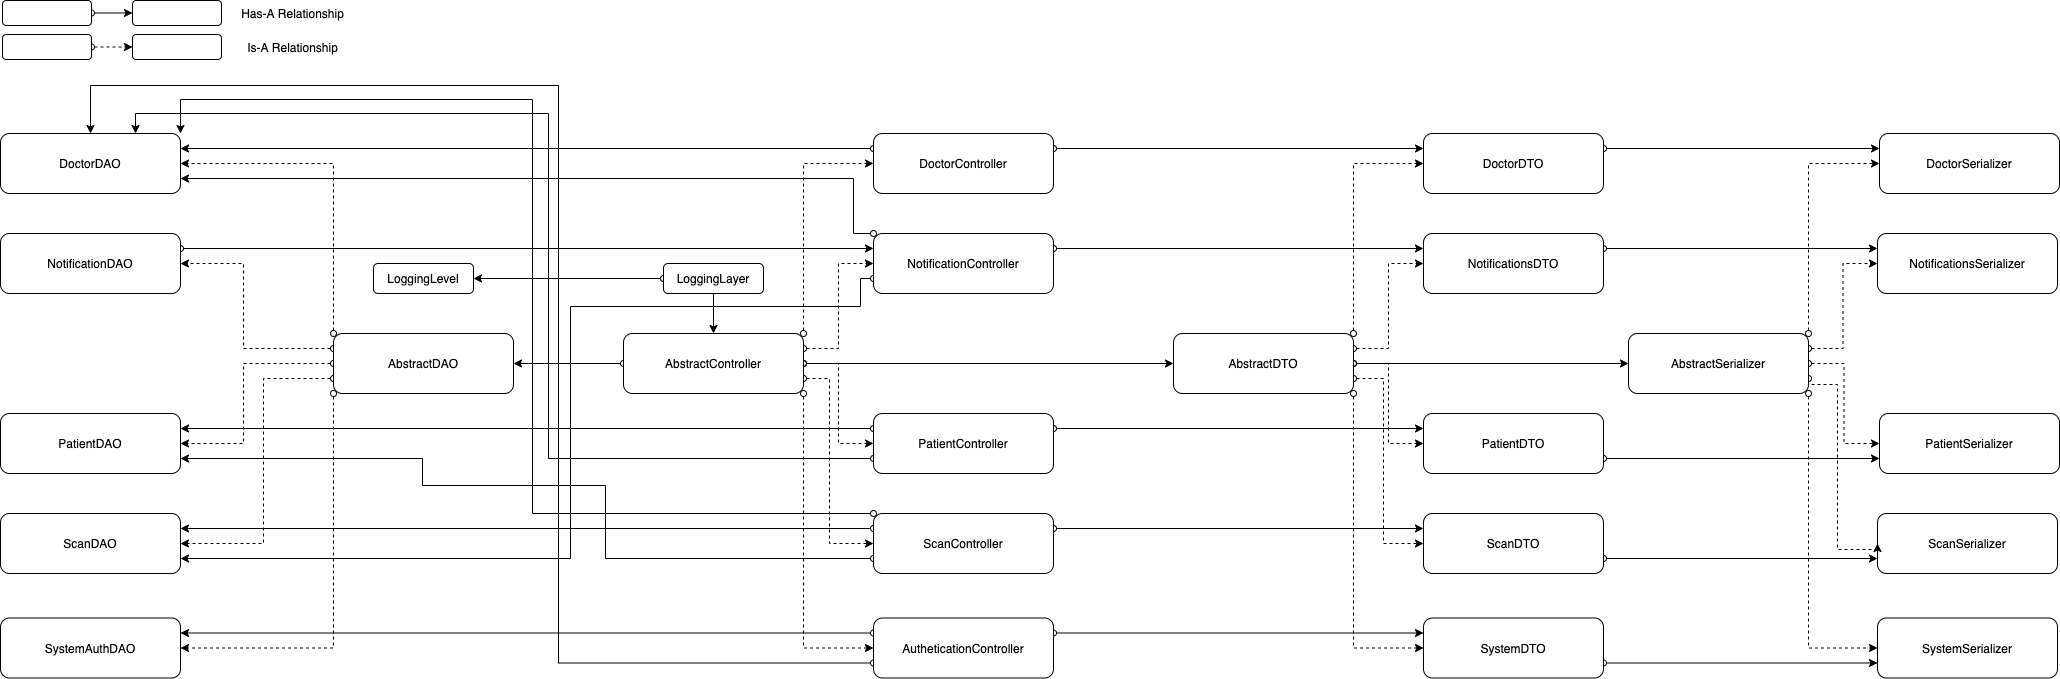
\includegraphics[angle=90,origin=c,scale=0.3]{figures/InformationServiceArchitecture}
			\fi
		\end{figure}\pagebreak
		The entrypoints for the requests, are the following classes
		\begin{itemize}
			\item \textbf{DoctorController}: This Class handles everything related to the Doctor Entity.
			\item \textbf{NotificationController} : This Class handles everything related to the Notification Entity.
			\item \textbf{PatientController} : This Class handles everything related to the Patient Entity.
			\item \textbf{ScanController} : This Class handles everything related to the Scan Entity.
			\item \textbf{AutheticationController} : This Class handles everything related to the Authentication service.
		\end{itemize}
		When a request is sent to the Information service, the proper Class is selected based on the request endpoint and details. 
		Then the respective class will use the rest of the classes services to perform the needed actions and respond to the request
		accordincly. A exhaustive list of the rest major classes are given below.
		\begin{center}
			\begin{tabular}{ |c|c| } 
				\hline
				DoctorDAO & Handles the SQL Queries of Doctor Entity \\
				NotificationDAO & Handles the SQL Queries of Notification Entity  \\\
				PatientDAO & Handles the SQL Queries of the Patient Entity\\
				ScanDAO & Handles the SQL Queries of the Scan Entity\\
				SystemAuthDAO & Handles the SQL Queries of the Authentication service\\
				AbstractDAO & Used to describe any DAO(Data Access Object) available\\
				LoggingLayer & Used by controllers to notify the operator in case of errors\\
				LoggingLevel &Used by LoggingLayer to describe the severity of an error\\
				AbstractController & Used to describe any controller available\\
				AbstractDTO & Used to describe any DTO(Data Transfer Object)'s available\\
				DoctorDTO & The responce objects for Doctor Entities\\
				NotificationsDTO & The responce objects for Notification Entities\\
				PatientDTO & The responce objects for Patient Entities\\
				ScanDTO & The responce objects for Scan Entities\\
				SystemDTO & The responce objects for Authentication Entities\\
				AbstractSerializer & Used to describe any serializer available\\
				DoctorSerializer & Used to convert Doctor DTO responce into JSON\\
				NotificationsSerializer & Used to convert Notification DTO responce into JSON\\
				ScanSerializer & Used to convert Scan DTO responce into JSON\\
				SystemSerializer & Used to convert SystemAuthDTO responce into JSON\\
				\hline
			\end{tabular}
		\end{center}
		\subsection{Database Medium}
		The Information Service uses an RDBMS(Relational Database Managment System)[\cite{friedrichsen_ruffolo_monk_starks_pratt_last_1995}] called Postgres. PostgreSQL is a open-source and 
		free relational database emphasizing on extensibility and SQL standard compliance. The relational diagram of the Information Service
		can be seen below.Additional information relating the E-R Diagram can be found in chapter \ref{entity-relation-analysis} \pagebreak
		\begin{figure}[H]
			\iftrue
			\caption{E-R Diagram}
			\centering
			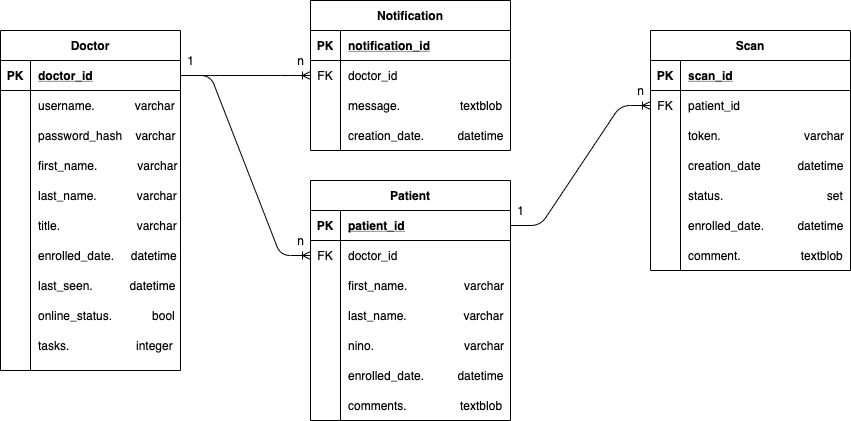
\includegraphics[angle=90,origin=c,scale=0.8]{figures/InformationServiceDatabaseDiagram}
			\fi
		\end{figure}\pagebreak
			
		